\documentclass{beamer}

\mode<presentation> {

% The Beamer class comes with a number of default slide themes
% which change the colors and layouts of slides. Below this is a list
% of all the themes, uncomment each in turn to see what they look like.

%\usetheme{default}
%\usetheme{AnnArbor}
%\usetheme{Antibes}
%\usetheme{Bergen}
%\usetheme{Berkeley}
%\usetheme{Berlin}
%\usetheme{Boadilla}
%\usetheme{CambridgeUS}
%\usetheme{Copenhagen}
%\usetheme{Darmstadt}
%\usetheme{Dresden}
%\usetheme{Frankfurt}
%\usetheme{Goettingen}
%\usetheme{Hannover}
%\usetheme{Ilmenau}
%\usetheme{JuanLesPins}
%\usetheme{Luebeck}
\usetheme{Madrid}
%\usetheme{Malmoe}
%\usetheme{Marburg}
%\usetheme{Montpellier}
%\usetheme{PaloAlto}
%\usetheme{Pittsburgh}
%\usetheme{Rochester}
%\usetheme{Singapore}
%\usetheme{Szeged}
%\usetheme{Warsaw}

% As well as themes, the Beamer class has a number of color themes
% for any slide theme. Uncomment each of these in turn to see how it
% changes the colors of your current slide theme.

%\usecolortheme{albatross}
%\usecolortheme{beaver}
%\usecolortheme{beetle}
%\usecolortheme{crane}
%\usecolortheme{dolphin}
%\usecolortheme{dove}
%\usecolortheme{fly}
%\usecolortheme{lily}
%\usecolortheme{orchid}
%\usecolortheme{rose}
%\usecolortheme{seagull}
%\usecolortheme{seahorse}
%\usecolortheme{whale}
%\usecolortheme{wolverine}

%\setbeamertemplate{footline} % To remove the footer line in all slides uncomment this line
%\setbeamertemplate{footline}[page number] % To replace the footer line in all slides with a simple slide count uncomment this line

%\setbeamertemplate{navigation symbols}{} % To remove the navigation symbols from the bottom of all slides uncomment this line
}

\usepackage{graphicx} % Allows including images
\usepackage{booktabs} % Allows the use of \toprule, \midrule and \bottomrule in tables

\usepackage{tikz}
\usetikzlibrary{arrows}


%----------------------------------------------------------------------------------------
%	TITLE PAGE
%----------------------------------------------------------------------------------------

\title[Robust MPC for Portfolio Optimization]{Robust Model Predictive Control for Portfolio Optimization} % The short title appears at the bottom of every slide, the full title is only on the title page

\author[M. Elibol, A. Kumar, E. Ratner, J. Sanz]{Melih Elibol, Ashish Kumar, Ellis Ratner, Josh Sanz} % Your name
\institute[] % Your institution as it will appear on the bottom of every slide, may be shorthand to save space
{
%University of California \\ % Your institution for the title page
\medskip
%\textit{john@smith.com} % Your email address
}
\date{\today} % Date, can be changed to a custom date

\begin{document}

\begin{frame}
\titlepage % Print the title page as the first slide
\end{frame}

\begin{frame}
\frametitle{Portfolio Optimization Problem}

    \begin{itemize}
    \item Empirical study comparing optimization models for investment strategies.
    \item We formulate the problem as three components
        \begin{enumerate}
        \item Asset value distribution

        \item Asset value predictor

        \item Investment strategy controller
        \end{enumerate}
    \end{itemize}

    \tikzstyle{int}=[draw, fill=blue!20, minimum size=2em]
\tikzstyle{init} = [pin edge={to-,thin,black}]

\begin{figure}
\centering
\begin{tikzpicture}[node distance=2.5cm,auto,>=latex']
    \node [int] (a) {Predictor};
    \node (b) [left of=a,node distance=4cm, coordinate] {a};
    \node [int] (c) [right of=a, node distance=3cm] {Controller};
    \node [coordinate] (end) [right of=c, node distance=2cm]{};
    \path[->] (b) edge node {$c_0, c_1, \dots, c_{t-1}$} (a);
    \path[->] (a) edge node {$\hat{c}_{t}$} (c);
    \draw[->] (c) edge node {$x_t$} (end) ;
\end{tikzpicture}
\end{figure}

\end{frame}

\begin{frame}
\frametitle{Asset Value Distributions}
    $c_t \in \mathbb{R}^n$ is the asset value at time $t$.
    \begin{block}{Stationary Gaussian Process}
        \[ c_t \sim \mathcal{N}\left(\mu, \Sigma \right) \]
    \end{block}
    \begin{block}{Linear Trending Gaussian Process}
        \[ c_t \sim \mathcal{N}\left(\mu_{t-1} + \Delta_\mu, \Sigma \right), \, \Delta_\mu \mbox{ fixed}\]
    \end{block}
    \begin{block}{Wiener Process}
        \[ c_t = c_{t-1} + u,\, u \sim \mathcal{N}\left(\mu, \Sigma \right) \]
    \end{block}

\end{frame}

\begin{frame}
\frametitle{Asset Value Predictors}

    $c_t \in \mathbb{R}^n$ is the asset value at time $t$.

    \begin{block}{Unbiased Estimator of Gaussians}
    \[ \hat{\mu} = \frac{1}{m} \sum_{i=1}^{m} c_i \hspace{1cm} \hat{\Sigma}_{jk} = \frac{1}{m-1} \sum_{i=1}^{m} (c_{ij} - \hat{\mu}_j)(c_{ik} - \hat{\mu}_k). \]
    \end{block}

    \begin{block}{Gaussian Estimator with Time Horizon $T$}
    \[ \hat{\mu} = \frac{1}{T} \sum_{i=m-T}^{m} c_i \hspace{1cm} \hat{\Sigma}_{jk} = \frac{1}{T-1} \sum_{i=m-T}^{m} (c_{ij} - \hat{\mu}_j)(c_{ik} - \hat{\mu}_k). \]
    \end{block}

    \begin{block}{Autoregressive Model}
    \[ c_t = \sum_{i=1}^p \theta_i c_{t-i} + \epsilon_t. \]
    \end{block}

\end{frame}

\begin{frame}
\frametitle{Investment Strategy Controllers}

    \begin{block}{L1 and L2 Regularization}
    \begin{align*}
        \max_{w\in\mathbb{R}^n}{} & \hat{c}^T w - \lambda \Vert w \Vert_L \\
        \mbox{s.t.} & \sum_{i=0}^{n} w_i \leq 1 \\
        & w_i \geq 0, i=1,...,n
    \end{align*}
    \end{block}

    \begin{center}
        Result from dualizing a norm-ball uncertainty set on $c$ \\
        \[ c \in \mathcal{U}=\left\{ c : \|\hat{c} - c\|_p \leq \lambda \right\} \]
    \end{center}

\end{frame}

\begin{frame}
\frametitle{Investment Strategy Controllers}

    \begin{block}{Weighted Regularization}
    \begin{align*}
        \max_{w\in\mathbb{R}^n}{} & \hat{c}^T w - \lambda (w^T \Sigma w) \\
        \mbox{s.t.} & \sum_{i=0}^{n} w_i \leq 1 \\
        & w_i \geq 0, i=1,...,n
    \end{align*}
    \end{block}


    \begin{center}
        Results from dualizing a weighted norm-ball uncertainty set on $c$ \\
        \[ c \in \mathcal{U}=\left\{ c : (\hat{c} - c)^T \Sigma^{-1}(\hat{c} - c) \leq \lambda \right\} \]
    \end{center}

\end{frame}

\begin{frame}
\frametitle{Experimental Results}

\begin{block}{Gaussian Noise Return Residuals}
    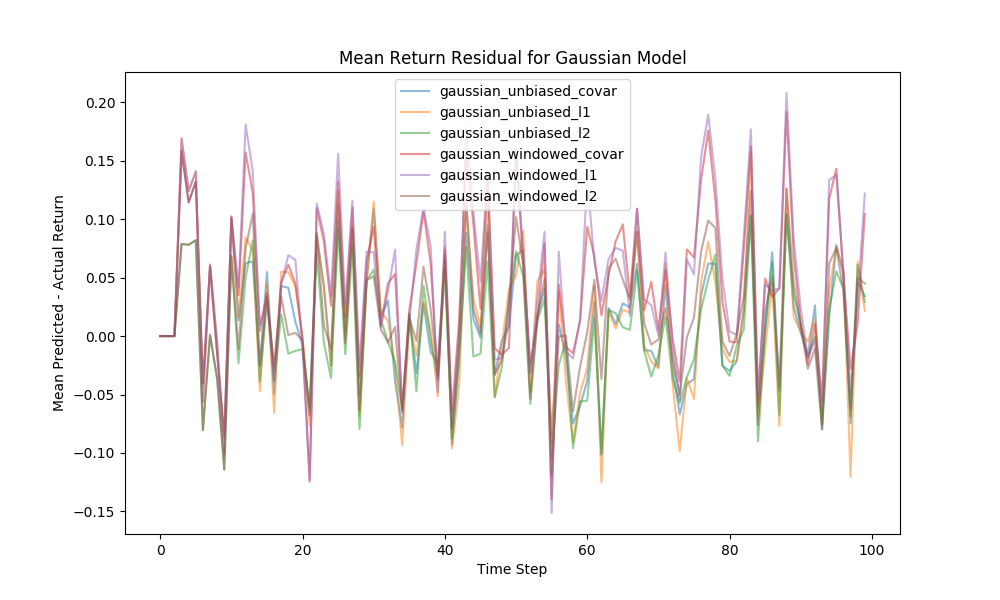
\includegraphics[width=\linewidth]{mean_return_residual-Gaussian_model.png}
\end{block}

\end{frame}

\begin{frame}
    \frametitle{Experimental Results}

    \begin{block}{Linear Trending Gaussian Return Residuals}
        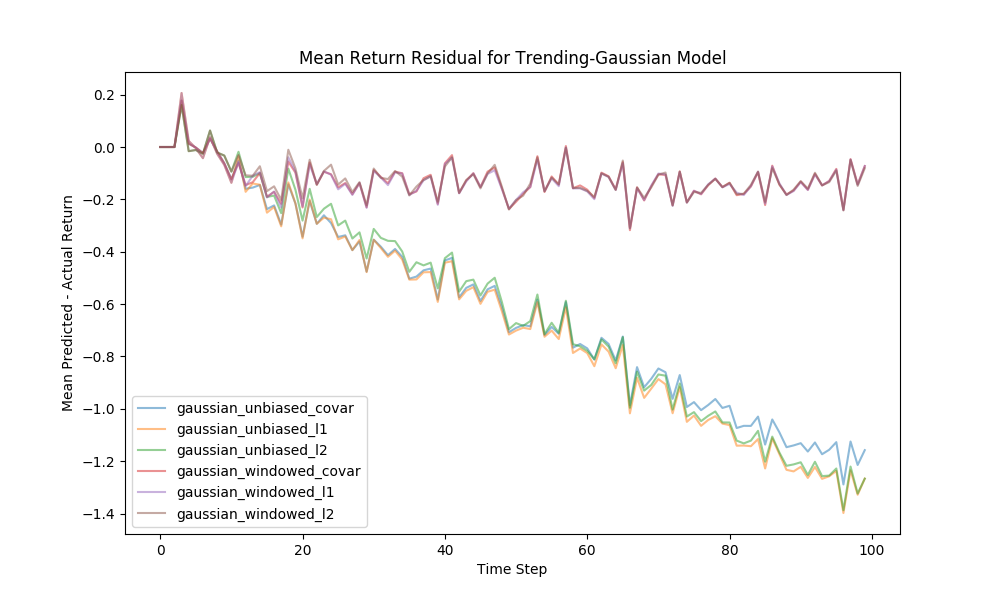
\includegraphics[width=\linewidth]{mean_return_residual-Trending-Gaussian_model.png}
    \end{block}

\end{frame}

\begin{frame}
    \frametitle{Experimental Results}

    \begin{block}{Wiener Process Return Residuals}
        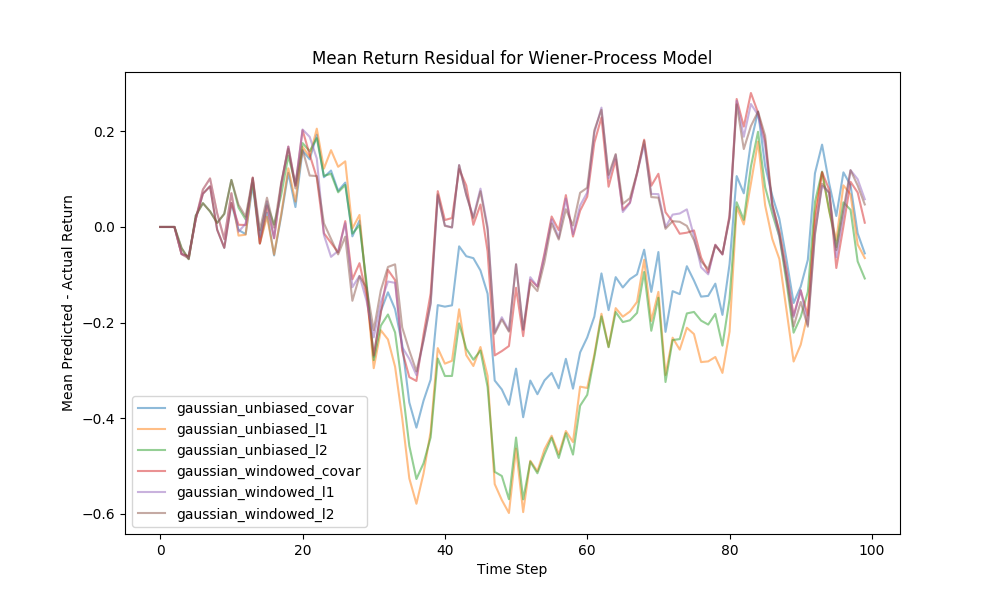
\includegraphics[width=\linewidth]{mean_return_residual-Wiener-Process_model.png}
    \end{block}

\end{frame}

\begin{frame}
    \frametitle{Experimental Results}

    \begin{block}{Gaussian Noise Regularization Parameter vs Return}
        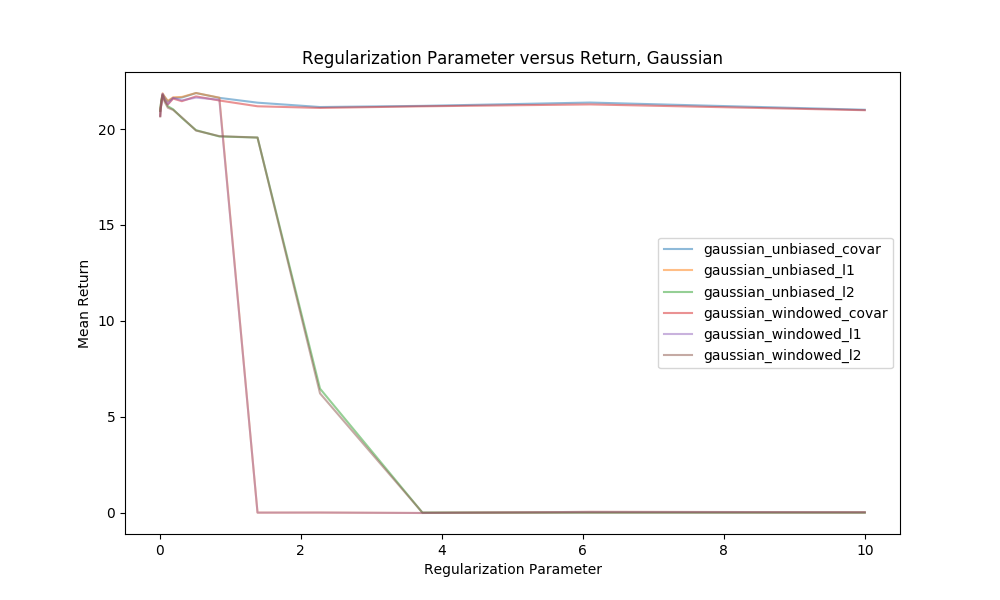
\includegraphics[width=\linewidth]{gammma_vs_return-Gaussian.png}
    \end{block}

\end{frame}

\begin{frame}
    \frametitle{Experimental Results}

    \begin{block}{Linear Trending Gaussian Regularizatio Parameter vs Return}
        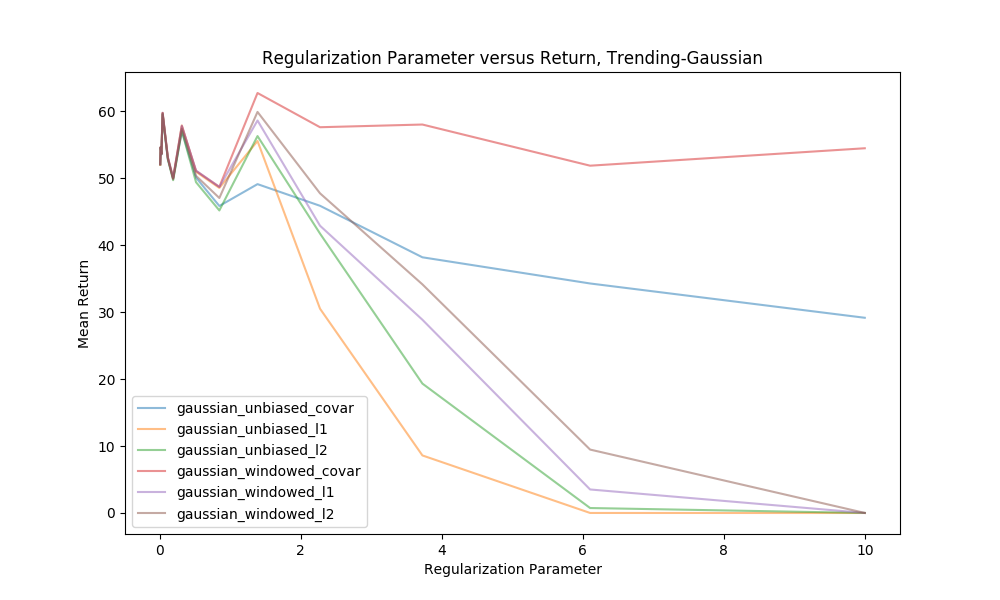
\includegraphics[width=\linewidth]{gammma_vs_return-Trending-Gaussian.png}
    \end{block}

\end{frame}

\begin{frame}
    \frametitle{Experimental Results}

    \begin{block}{Wiener Process Regularizatio Parameter vs Return}
        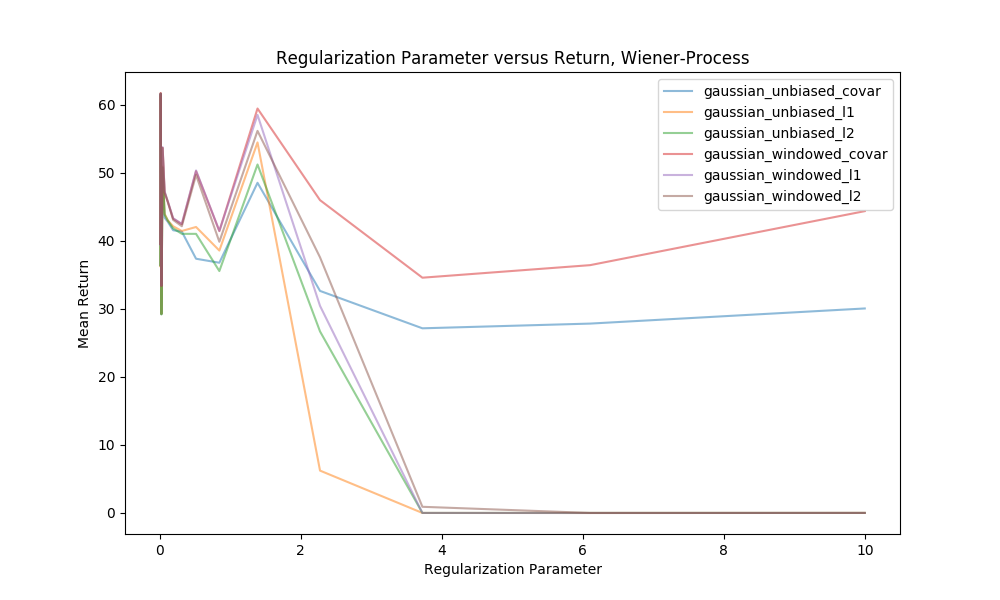
\includegraphics[width=\linewidth]{gammma_vs_return-Wiener-Process.png}
    \end{block}

\end{frame}



\begin{frame}
    \Huge{\centerline{Next Steps}}
\end{frame}


\begin{frame}
    \frametitle{Additional Asset Value Distribution Models}
    \begin{enumerate}
        \item Adversarial Noise
    \end{enumerate}
\end{frame}

\begin{frame}
    \frametitle{Additional Asset Value Predictor Models}

\end{frame}

\begin{frame}
    \frametitle{Additional Investment Control Models}

    \begin{itemize}
      \item Conditional Value at Risk (CVaR) constraint: enforces upper bound on probability of low return
        \begin{align*}
          \mathrm{P}\left\{c : \gamma \leq -w\tran c \right\} \leq \epsilon
        \end{align*}

      \item Robust MPC
    \end{itemize}

\end{frame}

\begin{frame}
    \Huge{\centerline{Questions?}}
\end{frame}

% %------------------------------------------------

% \begin{frame}
% \frametitle{Bullet Points}
% \begin{itemize}
% \item Lorem ipsum dolor sit amet, consectetur adipiscing elit
% \item Aliquam blandit faucibus nisi, sit amet dapibus enim tempus eu
% \item Nulla commodo, erat quis gravida posuere, elit lacus lobortis est, quis porttitor odio mauris at libero
% \item Nam cursus est eget velit posuere pellentesque
% \item Vestibulum faucibus velit a augue condimentum quis convallis nulla gravida
% \end{itemize}
% \end{frame}

% %------------------------------------------------

% \begin{frame}
% \frametitle{Blocks of Highlighted Text}
% \begin{block}{Block 1}
% Lorem ipsum dolor sit amet, consectetur adipiscing elit. Integer lectus nisl, ultricies in feugiat rutrum, porttitor sit amet augue. Aliquam ut tortor mauris. Sed volutpat ante purus, quis accumsan dolor.
% \end{block}

% \begin{block}{Block 2}
% Pellentesque sed tellus purus. Class aptent taciti sociosqu ad litora torquent per conubia nostra, per inceptos himenaeos. Vestibulum quis magna at risus dictum tempor eu vitae velit.
% \end{block}

% \begin{block}{Block 3}
% Suspendisse tincidunt sagittis gravida. Curabitur condimentum, enim sed venenatis rutrum, ipsum neque consectetur orci, sed blandit justo nisi ac lacus.
% \end{block}
% \end{frame}

% %------------------------------------------------

% \begin{frame}
% \frametitle{Multiple Columns}
% \begin{columns}[c] % The "c" option specifies centered vertical alignment while the "t" option is used for top vertical alignment

% \column{.45\textwidth} % Left column and width
% \textbf{Heading}
% \begin{enumerate}
% \item Statement
% \item Explanation
% \item Example
% \end{enumerate}

% \column{.5\textwidth} % Right column and width
% Lorem ipsum dolor sit amet, consectetur adipiscing elit. Integer lectus nisl, ultricies in feugiat rutrum, porttitor sit amet augue. Aliquam ut tortor mauris. Sed volutpat ante purus, quis accumsan dolor.

% \end{columns}
% \end{frame}

% %------------------------------------------------
% \section{Second Section}
% %------------------------------------------------

% \begin{frame}
% \frametitle{Table}
% \begin{table}
% \begin{tabular}{l l l}
% \toprule
% \textbf{Treatments} & \textbf{Response 1} & \textbf{Response 2}\\
% \midrule
% Treatment 1 & 0.0003262 & 0.562 \\
% Treatment 2 & 0.0015681 & 0.910 \\
% Treatment 3 & 0.0009271 & 0.296 \\
% \bottomrule
% \end{tabular}
% \caption{Table caption}
% \end{table}
% \end{frame}

% %------------------------------------------------

% \begin{frame}
% \frametitle{Theorem}
% \begin{theorem}[Mass--energy equivalence]
% $E = mc^2$
% \end{theorem}
% \end{frame}

% %------------------------------------------------

% \begin{frame}[fragile] % Need to use the fragile option when verbatim is used in the slide
% \frametitle{Verbatim}
% \begin{example}[Theorem Slide Code]
% \begin{verbatim}
% \begin{frame}
% \frametitle{Theorem}
% \begin{theorem}[Mass--energy equivalence]
% $E = mc^2$
% \end{theorem}
% \end{frame}\end{verbatim}
% \end{example}
% \end{frame}

% %------------------------------------------------

% \begin{frame}
% \frametitle{Figure}
% Uncomment the code on this slide to include your own image from the same directory as the template .TeX file.
% %\begin{figure}
% %\includegraphics[width=0.8\linewidth]{test}
% %\end{figure}
% \end{frame}

% %------------------------------------------------

% \begin{frame}[fragile] % Need to use the fragile option when verbatim is used in the slide
% \frametitle{Citation}
% An example of the \verb|\cite| command to cite within the presentation:\\~

% This statement requires citation \cite{p1}.
% \end{frame}

% %------------------------------------------------

% \begin{frame}
% \frametitle{References}
% \footnotesize{
% \begin{thebibliography}{99} % Beamer does not support BibTeX so references must be inserted manually as below
% \bibitem[Smith, 2012]{p1} John Smith (2012)
% \newblock Title of the publication
% \newblock \emph{Journal Name} 12(3), 45 -- 678.
% \end{thebibliography}
% }
% \end{frame}

% %------------------------------------------------

% \begin{frame}
% \Huge{\centerline{The End}}
% \end{frame}

%----------------------------------------------------------------------------------------

\end{document}